\chapter{Problem Motivation}

\section{Introduction}    

The volume of scientific literature has doubled in the past 20 years\footnote{https://data.worldbank.org/indicator/IP.JRN.ARTC.SC}.  
The ubiquity of computing and access to free, open-source software has also enabled exponential growth in publishing for computer science fields.  
Figure \ref{figure1} shows a plot of the number of papers published annually on computer science(CS) ArXiv\footnote{https://arxiv.org} each year 2015 to 2020 on a log scale. 

\begin{figure}[h]
    \centering
    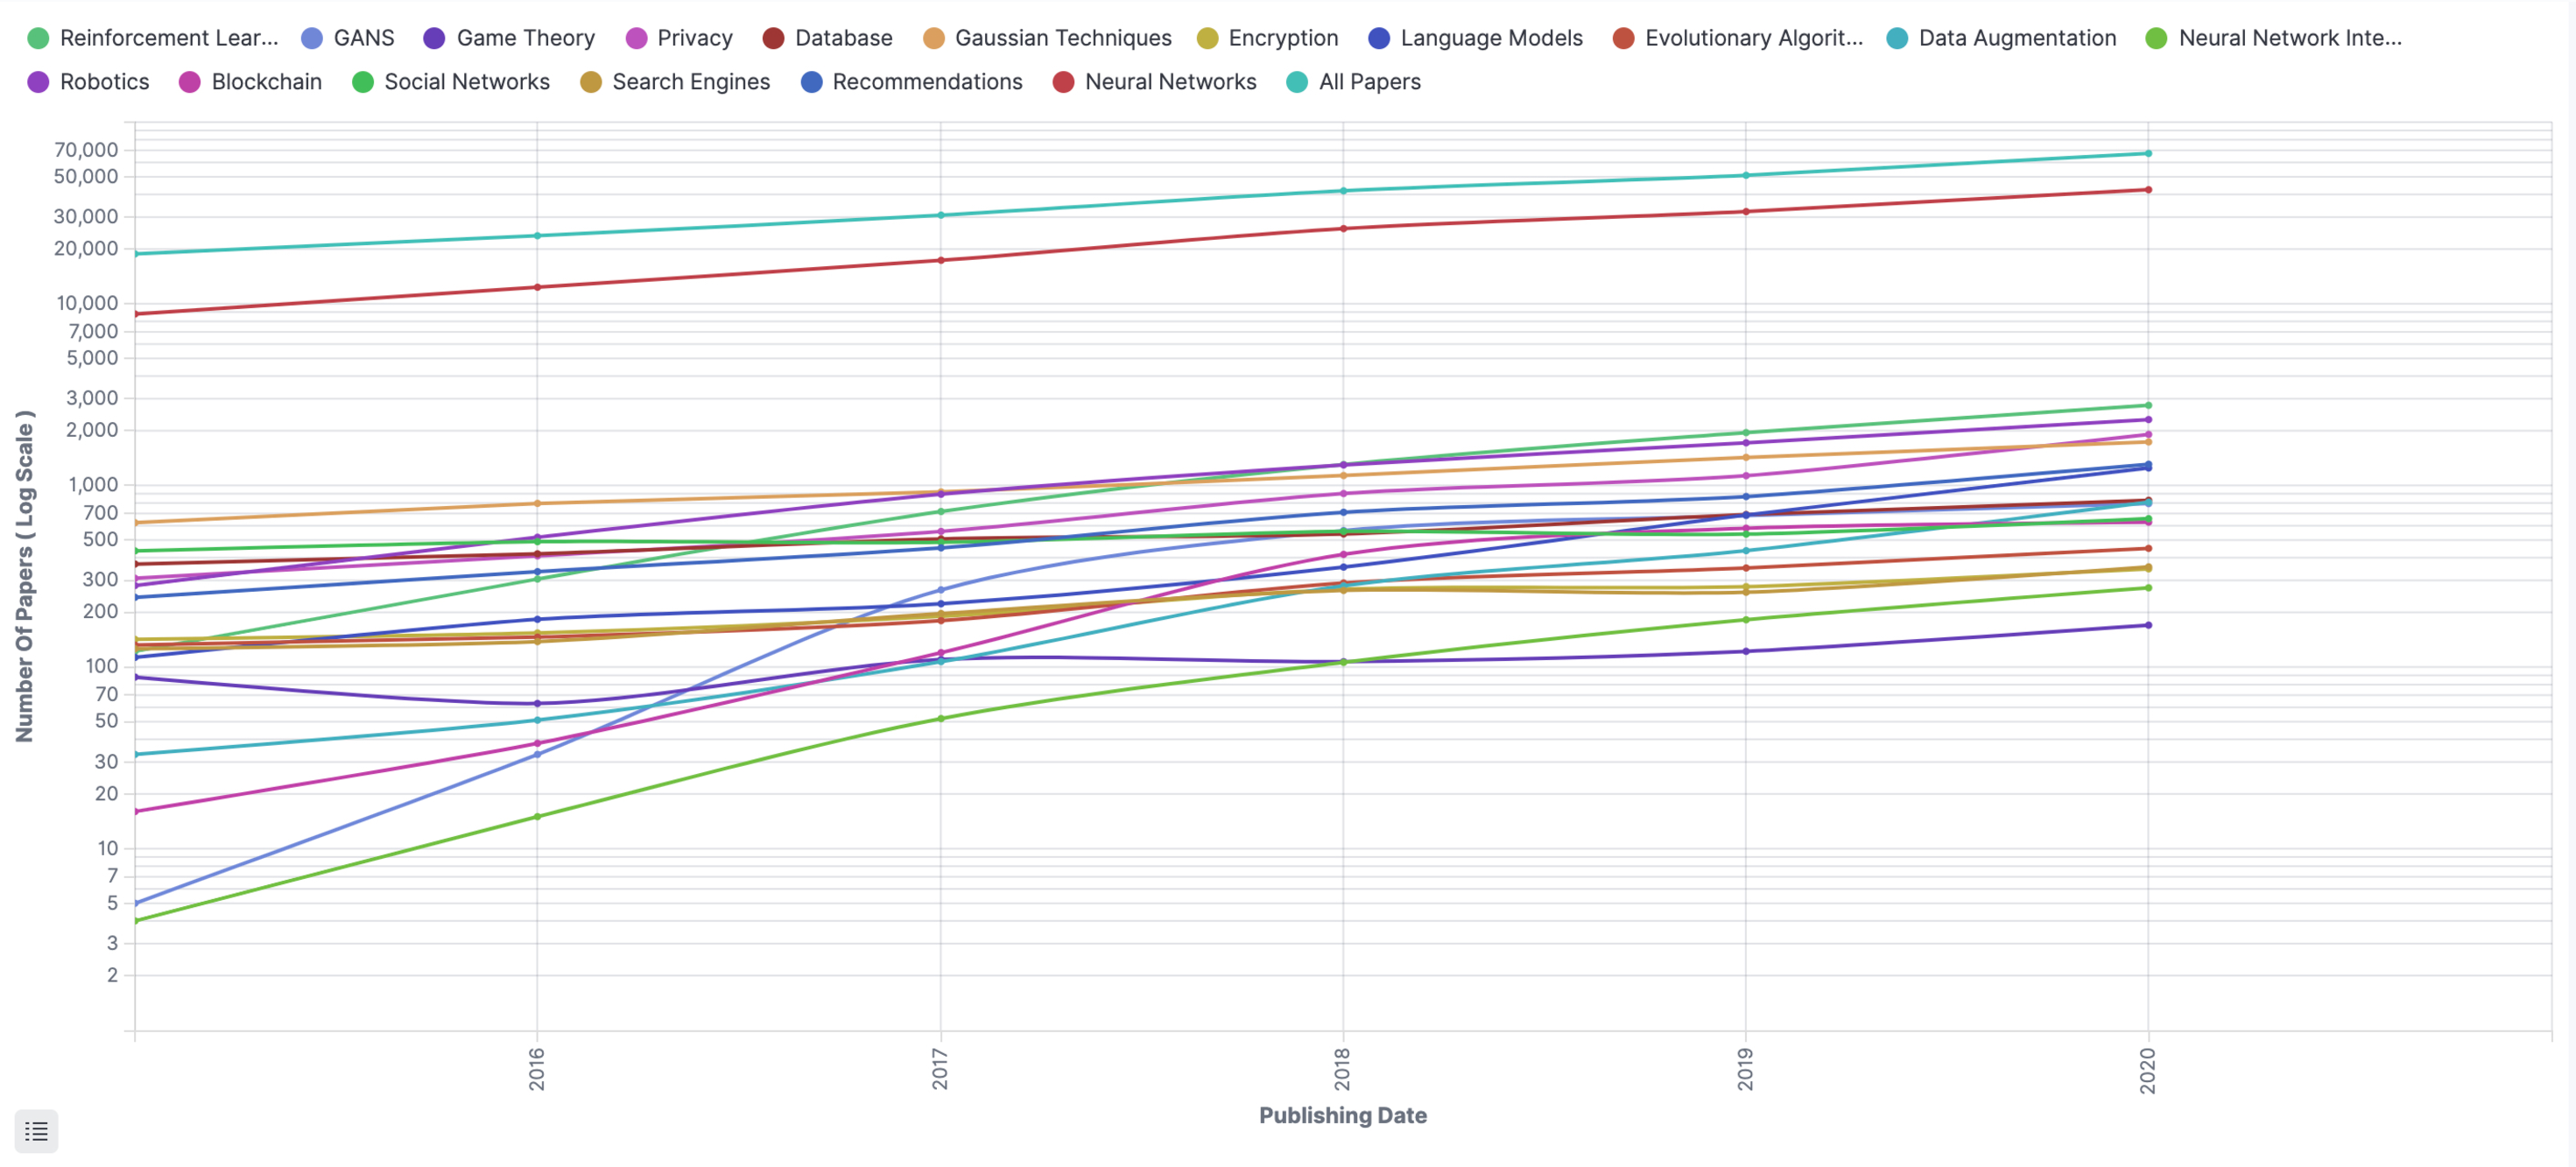
\includegraphics[width=\maxwidth{\textwidth}]{src/images/num-papers.pdf}
    \caption{ A time series plotting count of papers every year for across various topics in CS from January 2015 to December 2020}
    \label{figure\arabic{figurecounter}}
\end{figure}
\refstepcounter{figurecounter}

The growth in the research volume has also led to academic research search engines becoming primary mediums of access for scientific literature. 

Academic research search engines are different from traditional search engines like Google because they host content specific to scientific literature. 
Scientific papers generally undergo a process of peer-review. If a paper does not undergo peer review, it may still get cited by other publications/articles. This relational nature of academic research makes it relatively easy to filter credibility based on citations as a metric; Major academic research search engines such as Google Scholar, Microsoft Academic, etc., leverage citations as a metric for ranking documents. Although citations are beneficial, a search query may match many records during the search process. The increase in the number of documents can also result in a sea of noise for a particular search query. In such cases, the researcher gets minimal context information around search matches to infer the usefulness of a search result. 

Researchers also tend to look for information embedded deep inside papers. Many papers contain table/s of results for some experiments or comparisons to techniques/methods from other papers. The methods/techniques that are compared are generally cited; But the access to thier information requires researchers to manually hunt for the information to drive context behind the comparison. This type of tabular information is not easily accessible through normal search engines. It is also not readily available at the time of reading research. A platform like PapersWithCode\footnote{https://paperswithcode.com} hosts/tracks State-of-the-art(SOTA) leaderboards for Machine Learning(ML) along with their papers. The access to information within this platform is constrained to ML and doesn't provide information outside papers in Machine Learning papers. 

The next section aims to provide a motivating example to explain the lack of context in search results displayed by three large proprietary search engines.

\section{Motivating Example: Search Results From Academic Research Search Engines}
Machine Learning and deep learning research dominate most CS publications on pre-print servers like ArXiv (Figure \ref{figure1}).
Based on this information, consider the use-case of a researcher trying to look for papers where a Transformer\parencite{vaswani2017attention} model written in PyTorch\parencite{paszke2019pytorch} is given adversarial examples. 
The researcher chooses to use the following search query: \textit{pytorch transformer adversarial examples} on the search engines Google Scholar, Semantic Scholar, and Microsoft Academic. 
Ideally, the experiments or the appendix or the methodology section of a paper would consist of information about code/model in a paper. 
The following subsections will analyze the search results for this query for three large search engines: Google Scholar, Microsoft Academic, and Semantic Scholar. 
\pagebreak
\subsection{Search Results From Google Scholar}
\label{sr-g}

\begin{figure}[h]
    \centering
    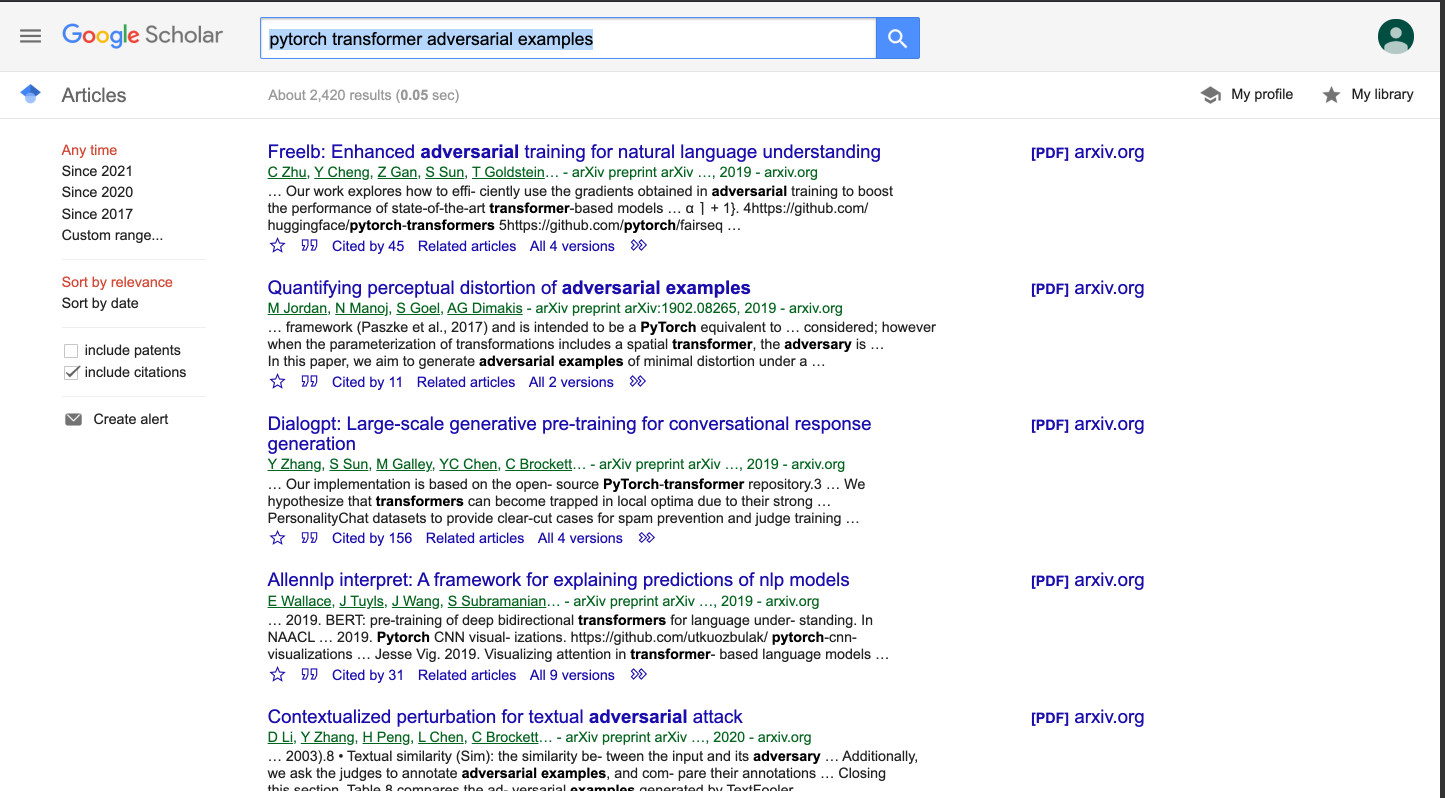
\includegraphics[width=\maxwidth{\textwidth}]{src/images/google-scholar-example.png}
    \caption{Search Results For Google Scholar}
    \label{figure\arabic{figurecounter}}
\end{figure}
\refstepcounter{figurecounter}
Although Google scholar found 2000+ search results, the search-result-fragments do not provide any additional context information about where the terms are matching.  There is no other context information except for links highlighted in the search results i.e., No mention of why the fragment matched. 

\pagebreak
\subsection{Search Results From Microsoft Academic}
\label{sr-m}
\begin{figure}[h]
    \centering
    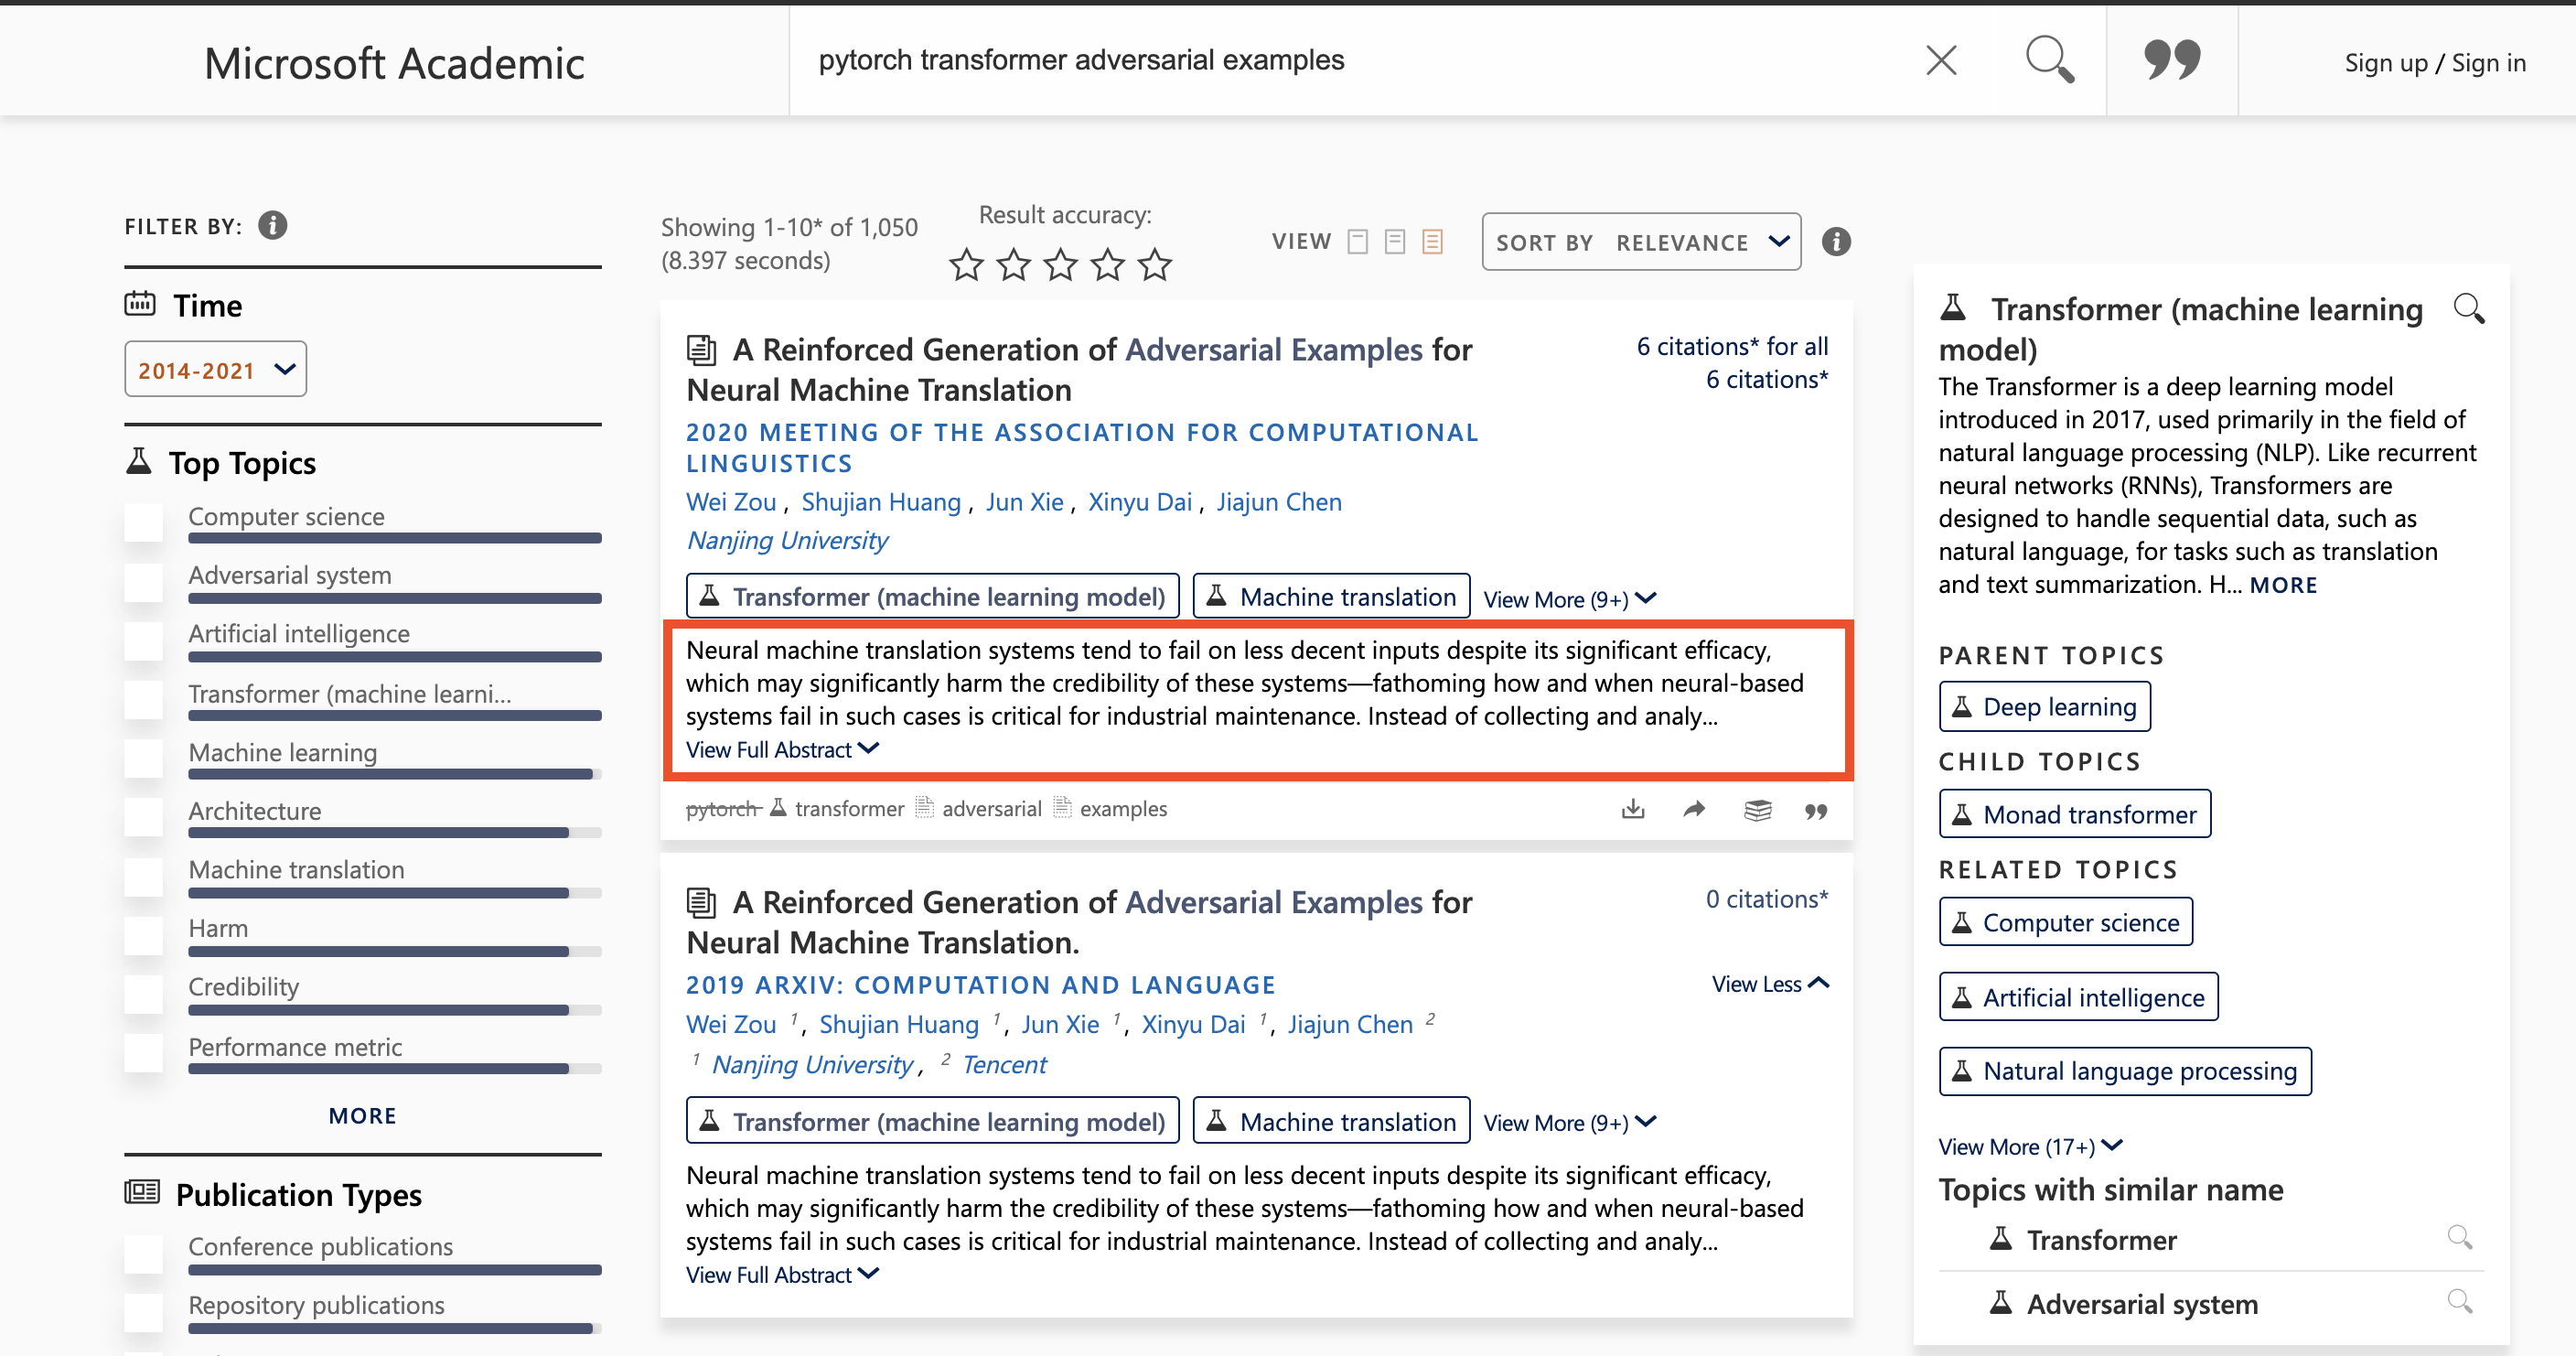
\includegraphics[width=\maxwidth{\textwidth}]{src/images/academic-example.png}
    \caption{Search Results For Microsoft Academic}
    \label{figure\arabic{figurecounter}}
\end{figure}
\refstepcounter{figurecounter}

Microsoft Academic provides additional information around context like topics, analytics on types of publication matches etc,
It fails to provide information about where the match took place in the paper.

\pagebreak
\subsection{Search Results From Semantic Scholar}
\label{sr-s}
\begin{figure}[h]
    \centering
    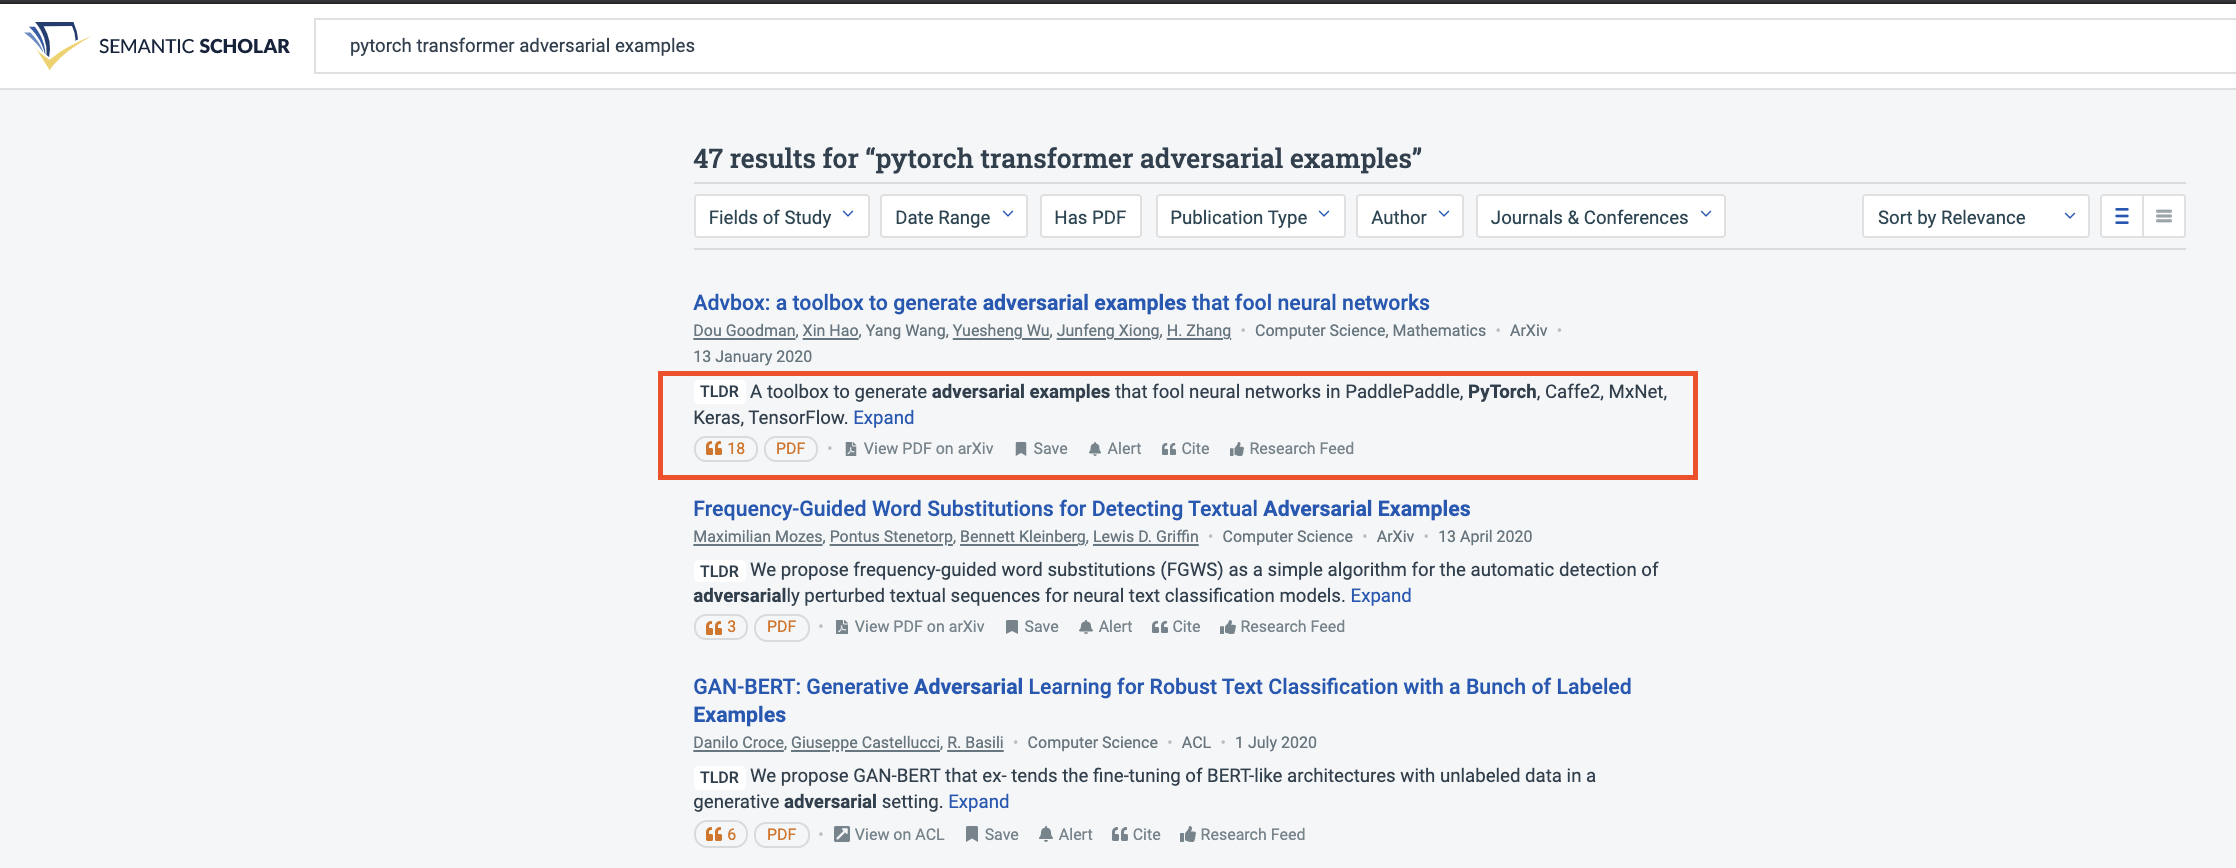
\includegraphics[width=\maxwidth{\textwidth}]{src/images/ss-example.png}
    \caption{Search Results For Semantic Scholar}
    \label{figure\arabic{figurecounter}}
\end{figure}
\refstepcounter{figurecounter}
Semantic Scholar highlights few search fragments where results would have matched and presented a smaller result set. 
But all search results do not consist of context about where the match took place. 

\pagebreak
\section{Characterizing Missing Traits}
\label{section:intro:missing_traits}

\subsection{Sparse Context In Search Results About Where Search Terms Matched Inside A Document}

All search results shown in section \ref{sr-g}, \ref{sr-m}, \ref{sr-s}, do not provide any additional information about where the match took place inside the research document. The interesting characteristic of research documents is that they possess structure and hierarchy. Research documents have well-laid out sections such as “Introduction,” “Related Works,” “Methodology,” “Experiments,” etc. that can provide context about the matched search terms. Such information can provide insights to the researcher about the context around which the search match took place. 

Previous studies by \parencite{kacem2018analysis} have shown that providing more filters to tend to improve precision in search. Access to the structure of the document can help the search engine provide filters to limit search within particular sections of a paper.

\pagebreak
\subsection{Minimal Access To Information When Reading Research}

\begin{figure}[h]
    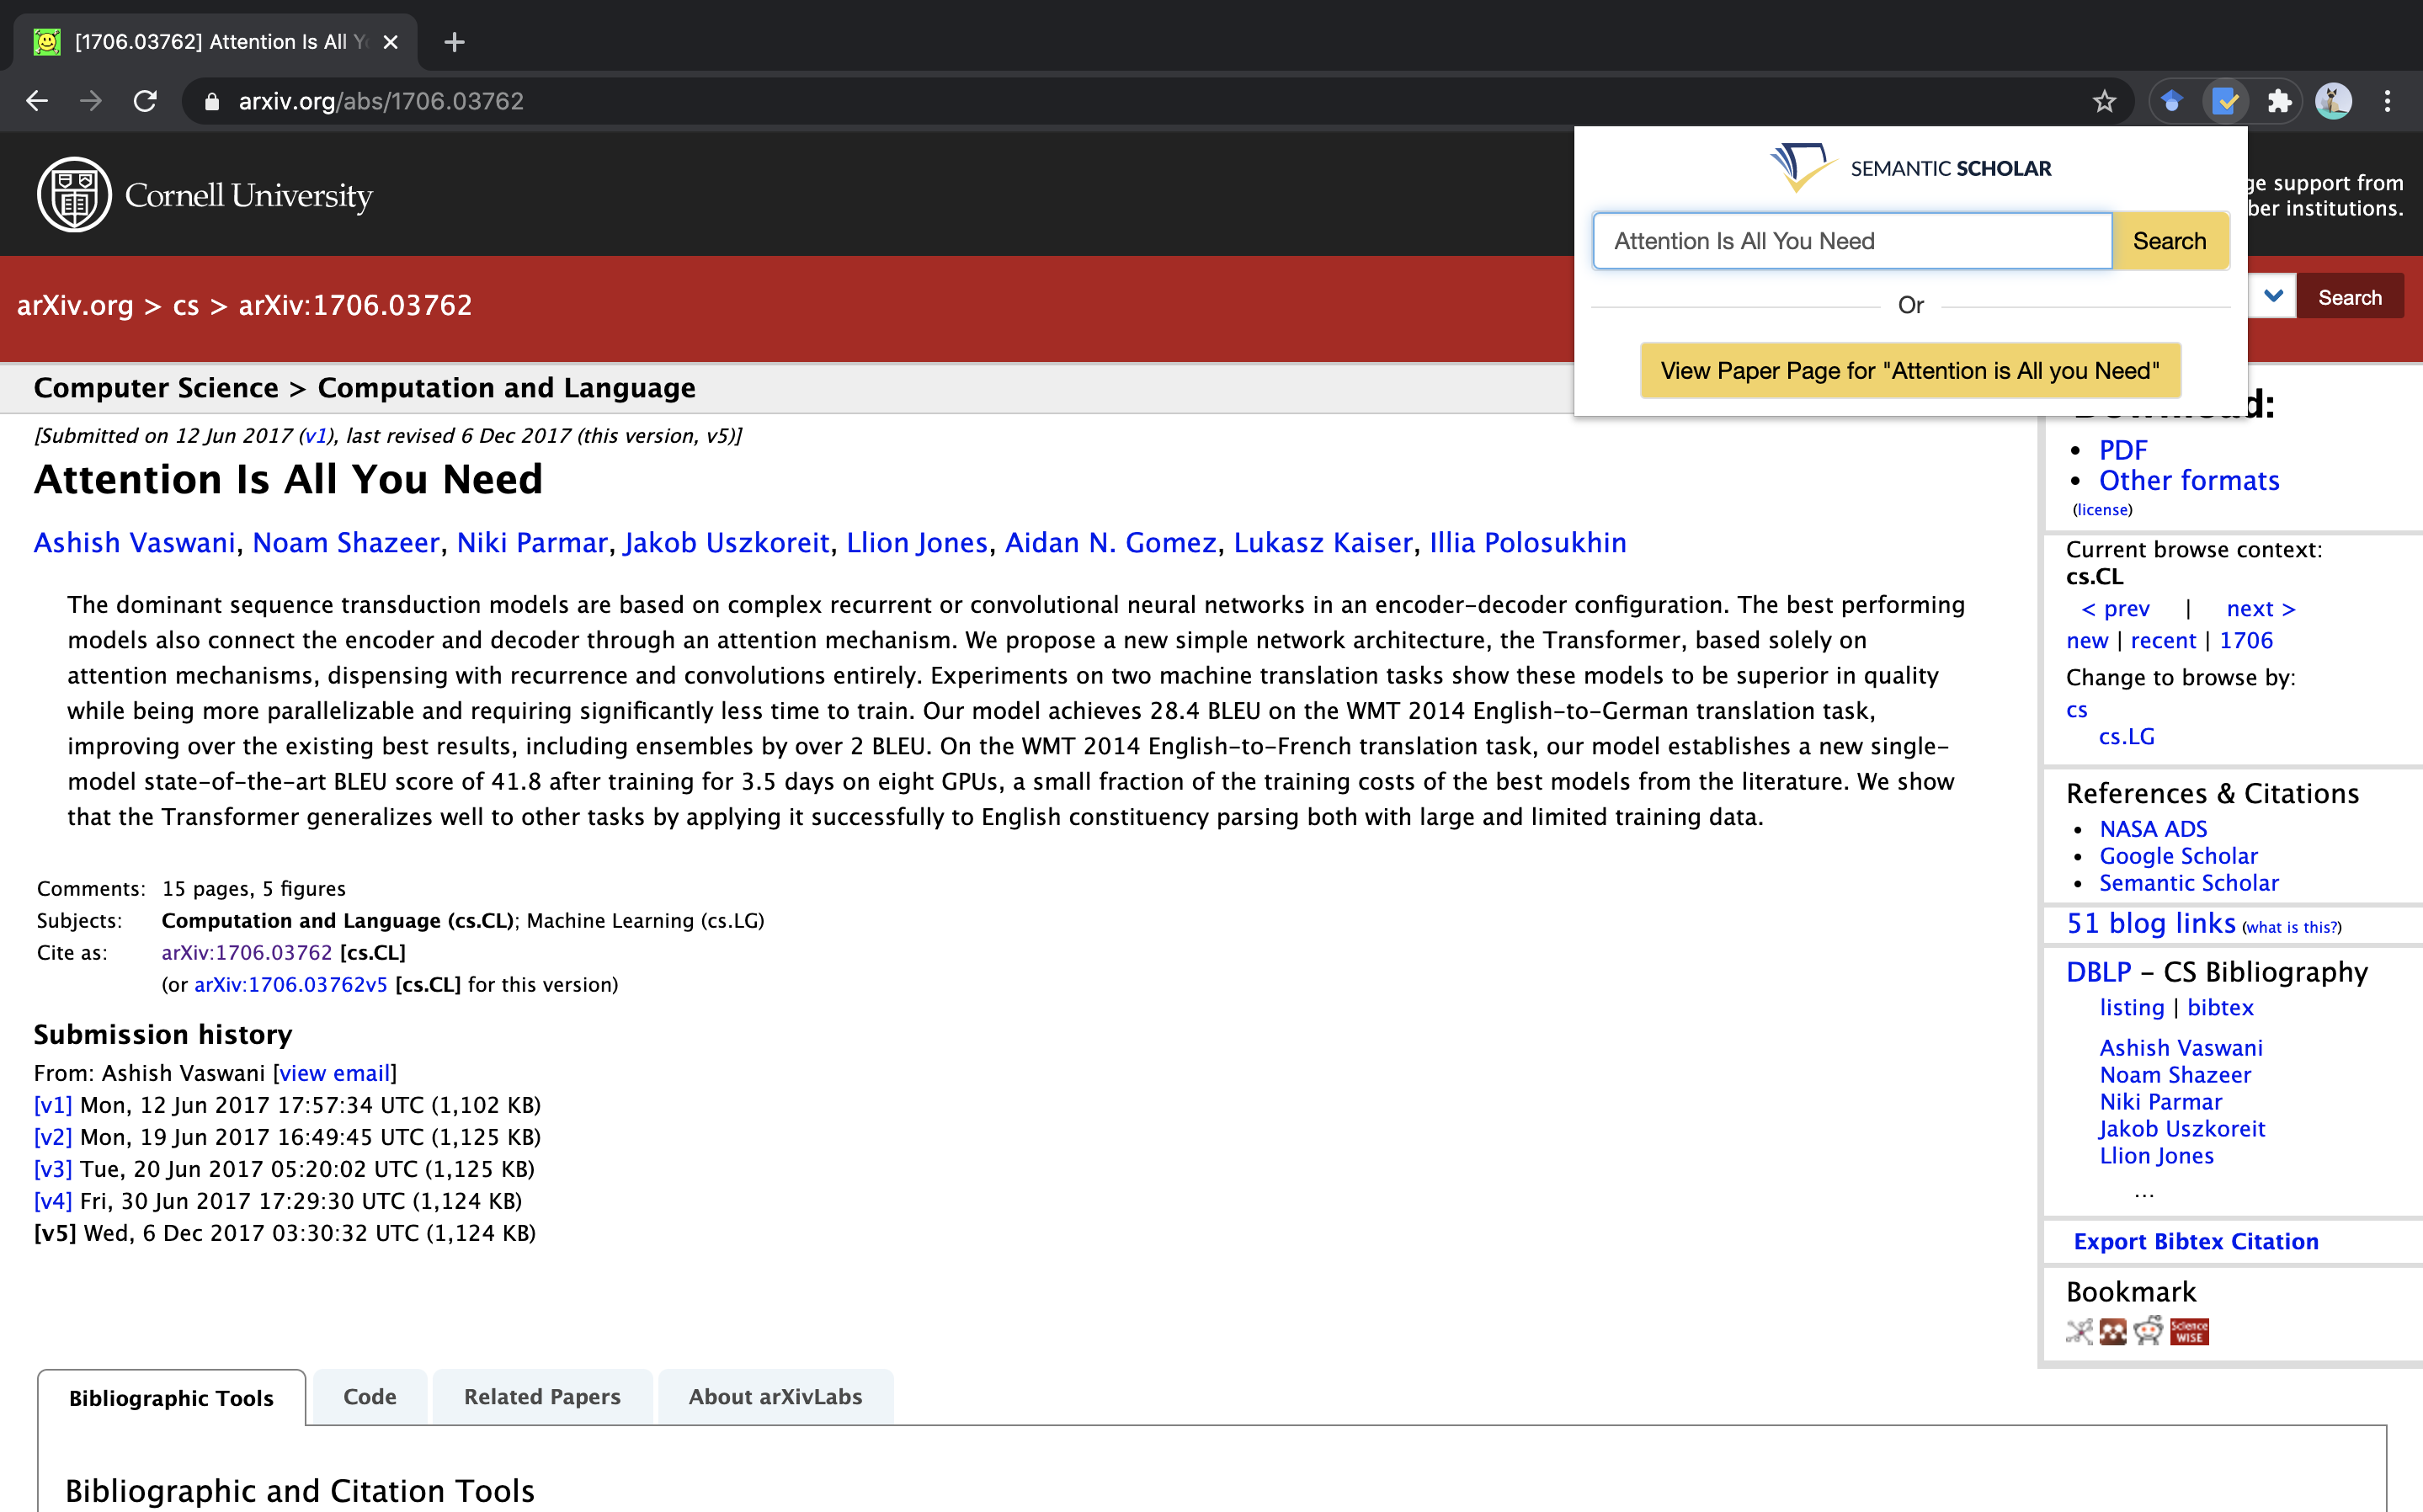
\includegraphics[width=0.475\textwidth]{src/images/gg-plugin.png}
    \hfill
    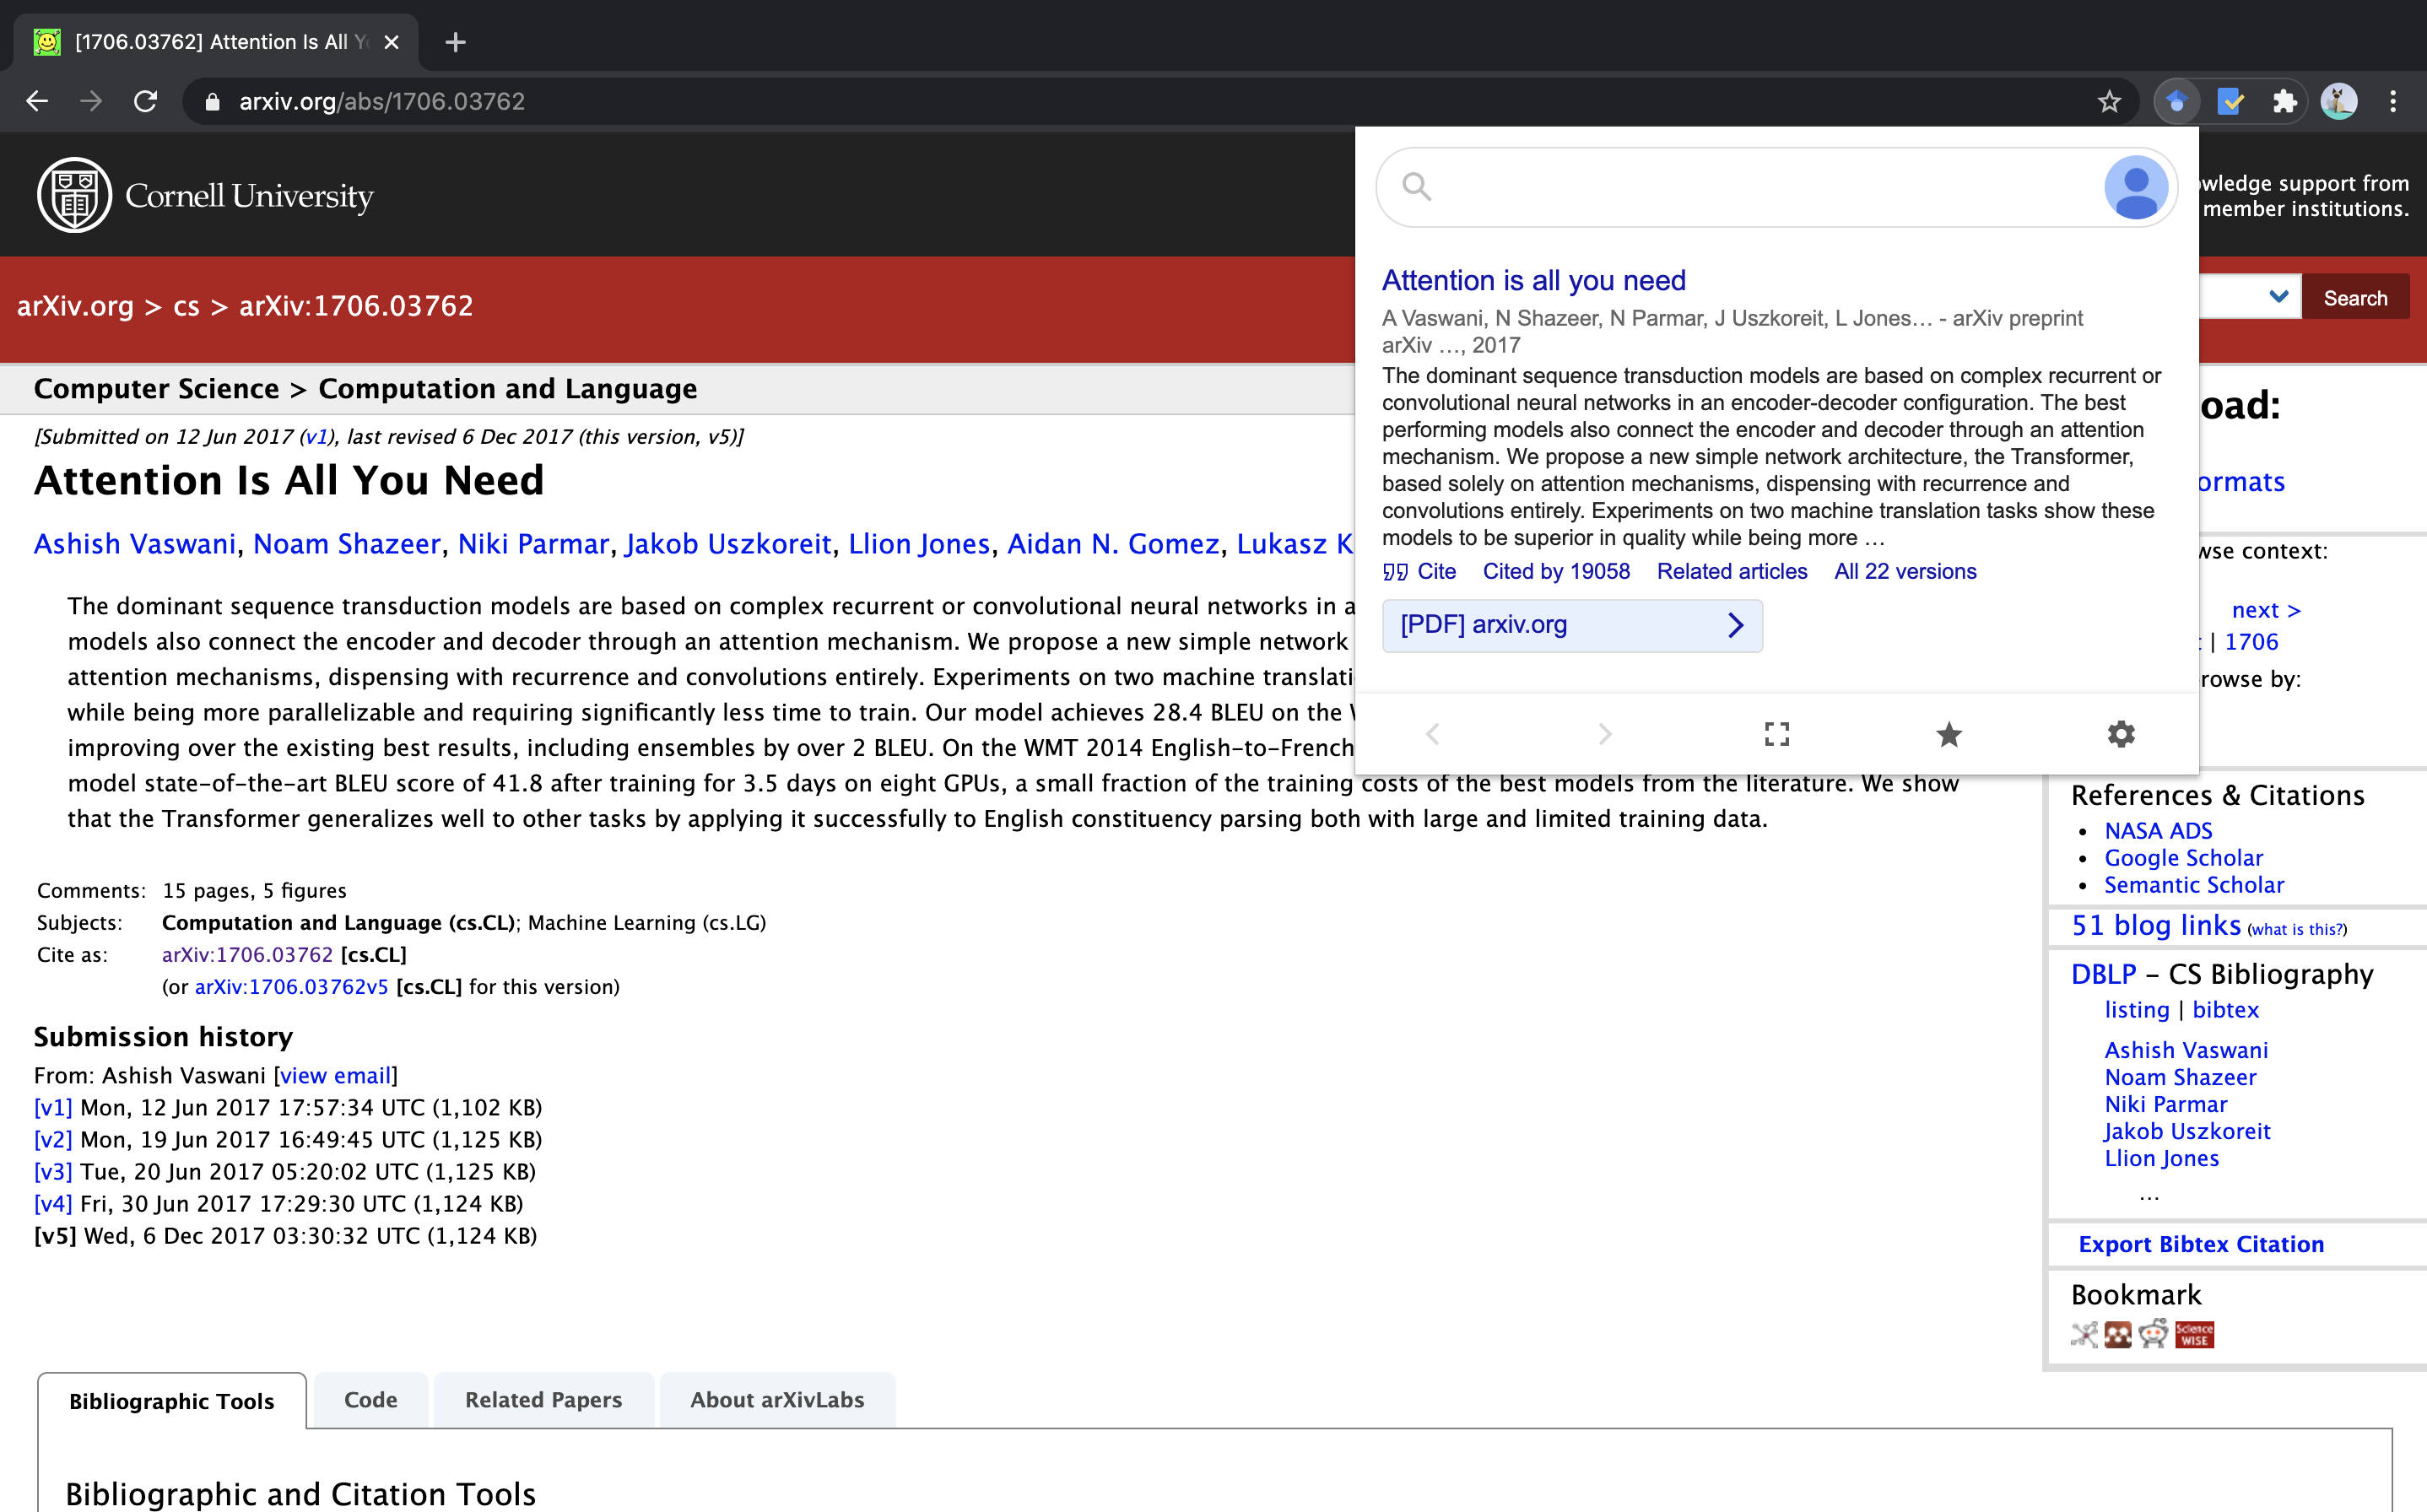
\includegraphics[width=0.475\textwidth]{src/images/ss-plugin.png}
    \caption{ Google Scholar and Semantic Scholar Plugins }
    \label{figure\arabic{figurecounter}}
\end{figure}
\refstepcounter{figurecounter}
Quite a few scientific literature search engines also offer forward citation search features \parencite{gusenbauer2020academic}, but these features are not always accessible outside the search engine’s website. 
Google Scholar and Semantic Scholar provide browser extensions to help the researchers get more context on a research document, as seen from Figure \ref{figure5}. 
These extensions lead back to the search engine's proprietary websites for further access to more information surrounding the research. They also do not provide information within the browser when the researcher is reading an article online. 
% They also miss out on many essential aspects of research documents, such as tables in the research when surfacing relevant information about the document. 
\subsection{No Access To More Fine-Grained Information Such as Tables When Reading Research}
\begin{figure}[h]
    \centering
    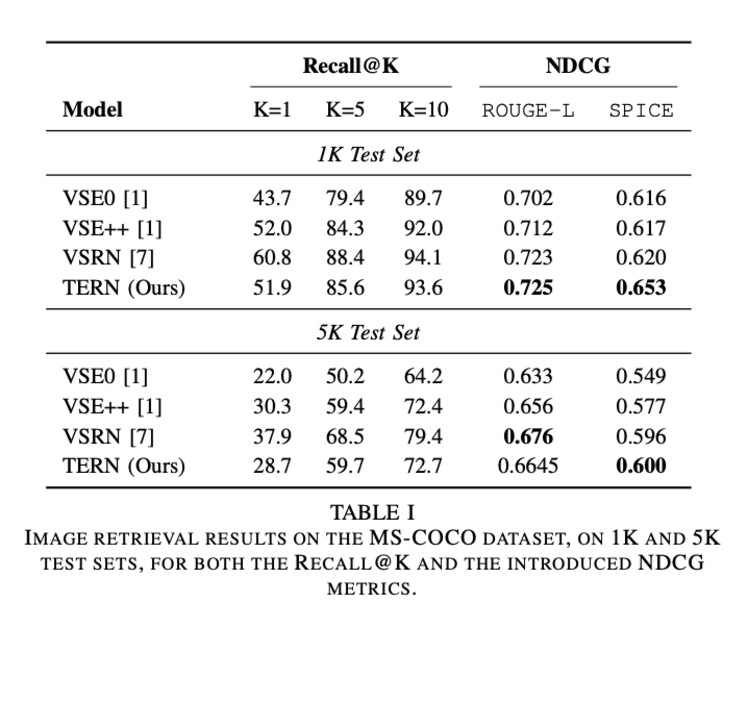
\includegraphics[width=\maxwidth{\textwidth}]{src/images/table-example.pdf}
    \legend{\emph{Source}: From \cite{messina2020transformer}}
    \caption{A table showing comparison of methods}
    \label{figure\arabic{figurecounter}}
\end{figure}
\refstepcounter{figurecounter}
Many research papers compare methods from other research papers, and such information is not directly accessible to the researcher when reading a research article online. Figure \ref{figure7} is a good example of a table showing comparison of methods. This table is derived from \cite{messina2020transformer}, and it describes comparisons with various methods; One of the method(VSRN) comes from \cite{li2019visual}. As comparisons are on the MS-COCO dataset \parencite{lin2014microsoft}, the user has to manually hunt for VSRN's performance from its original paper to understand variance in the method's performance from what was initially reported. This task of discovering tables with comparisons is a time-consuming task in research which requires a lot of mannual effort by a researcher.  

With the recent growth in Machine Learning publications, new platforms such as PapersWithCode\footnote{https://paperswithcode.com} and sotabench\footnote{https://sotabench.com/} help compare State-of-the-art(SOTA) methods from various research papers and link source code to many SOTA ML techniques. Even though these platforms host parsed information from raw research about comparsions with SOTA methods, there is no way to access that information when reading a research paper online. 

\section{Proposed Approach And Overview}
This dissertation focuses on the solutions developed to tackle the missing characteristics described in Section \ref{section:intro:missing_traits}. 

Section \ref{relatedwork:background} provides some preliminary background on inverted-index based search engines, open-source search engines, and state-of-the-art machine learning techniques.
Section \ref{relatedwork:acad-search-engine} discusses the different studies conducted about academic search engines; Section \ref{relatedwork:acad-lit-mining} discusses the different techniques used for mining academic literature; Section \ref{relatedwork:table-type} will discuss previous research to pertaining to classification of tables. 

Section \ref{method} provides an overview of the proposed solutions i.e., a search engine over CS ArXiv and a browser extension to augment research at the time of reading 

Section \ref{sci-genie-core} discusses the core components of the search engine and the browser extension; Section \ref{table_classification}
discusses the problem/application/experiments for table of comparison classification task.

Finally, Section \ref{conclusion} will provide some insight to the current shortcomings of Sci-Genie, highlight some future directions of research based on the shortcomings of Sci-Genie. 